\section{Signal processing}

\subsection{Overview of the system architecture}
The signal processing back-end of the CENT system was implemented using the open-souce OpenViBE platform \cite{renard2010openvibe}. The OpenViBE platform consists of a visual modelling language (similar to LabView or Simulink) which enables the design of various signal processing protocols which are called scenarios in the OpenViBE terminology. The scenarios can be drawn by connecting boxes representing various operations to each other in order to produce to a flowchart of how the data is processed. CENT integrates a fully functional version of OpenViBE which means that the original editor can be used to design new protocols or to modify the existing ones.

The signal processing back-end of the CENT system contains multiple OpenViBE scenarios. A list of scenarios required for a typical neurofeedback session can be found in table \ref{scenariolist}. Scenario-files can be found \textit{scenarios} subfolder of the CENT installation. Scenarios themselves are constructed using existing modules known as 'Boxes'. Boxes range from very simple (such as squaring each signal value) to more advanced (such as linear discrimant analysis or support vector machine classifications). Information between boxes is passed as streams of data. OpenViBE has multiple different streams but the two most important for the CENT system are 'Signals' and 'Stimulations'. Signals are simply chunks of EEG data that contain a buffer of the raw voltage values and the sampling rate used to acquire them. Stimulations are similar to trigger codes in most EEG applications and can be used to convey meta information like classification results or signal quality. Most of the common EEG signal analysis operations can be completed using a different combination of available boxes and streams. It is important to note that due to the open source nature of OpenViBE it is also possible to write new boxes for desired functionality.

\begin{table}[h]
\centering
\begin{tabular}{ll}
	\hline
	cent\_monitoring\_and\_noise.xml & Scenario for online monitoring of the 
	signal and checking the signal quality \\
	\hline
	cent\_baseline.xml & Baseline measurement \\
	\hline
	cent\_generate\_configuration.xml & A utlity sceneario used to generate configuration files required for the actual session \\
	\hline
	cent\_game.xml & The main scenario for the therapy session \\
	\hline
\end{tabular}
    \caption{List of OpenViBE scenarios used in CENT}\label{scenariolist}
\end{table}

Parameters for different boxes can either be set manually in the designer or they can be specified in a separate XML configuration file. Functionality of OpenViBE scenarios can be expanded using scripts written in Lua or Python languages. For more detailed explanation of box configuration see section GG.

Although box system is very flexible and grants much freedom in experiment design the implementations of even simple routines tend to be large. For example feature extraction of signal powers from few frequency bands can require the use of multiple boxes. Furthermore the implementation of these processes requires a certain level of knowledge regarding signal processing and might not be intuitive to the end user. For this reason to end user will not need to modify the OpenViBE scenarios in order to use the CENT system. Most of the necessary changes to the parameters can be done from within the CENT system and through configuration files.

The overall aim of the signal processing back-end is to classify the mental state of the patient to ADHD and non-ADHD based on the power modulations of theta and beta power bands of the EEG. In practice this is done by first acquiring a baseline recording of the theta and beta powers. Baseline is 60 second EEG recording where patient is just sitting still and staring at the fixation cross displayed on the monitor. In the subsequent game session the current power values of theta and beta are compared to the baseline values to determine shifts in the mental state. According to literature ADHD patient have excessive activity in the theta band and lower than average activity in the beta band. The desired effect is thus a decrease in beta and an increase in beta band. The change (whether positive or negative) is registered by the signal analysis module and passed back to the CENT system. The behaviour of the game is then modified based on this classification result. The patient receives the feedback as either success or failure in the game and thus slowly learns to modify their neural patterns.

This section briefly describes the operation of each of the scenario files. Each scenario can be divided into functional subelements that correspond to a certain step in a typical BCI processing chain. More information on the behaviour of the subelements can be found in the Signal processing protocol section, where structure and behaviour of different components are described.

\paragraph{Monitoring and noise}
Monitoring scenario is responsible for displaying the live EEG and current noise level at the beginning of the therapy session. This scenario is mainly a tool for making sure that the electrodes are properly fixed and that the data streaming is working. Figure \ref{monitoringnoise} shows the structure of the scenario. The scenario structure is relatively simple consisting only of acquisition client, filters and a noise calculator. The same structure is also used inside baseline and game scenarios.

\begin{figure}[h]
	\centering
	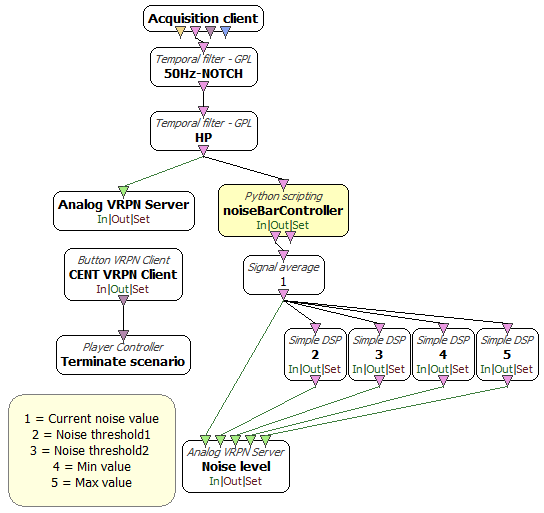
\includegraphics[scale=0.4]{noise.png}
	\caption{OpenViBE scenario for signal and noise check.}\label{monitoringnoise}
\end{figure}  

\paragraph{Baseline}
Baseline scenario is used to determine the baseline values for theta and beta power bands. During the baseline recording patient will be fixating on a cross displayed by the CENT system. Therapist screen will display the live EEG as well as the noise bar. Duration of the baseline recording is 60 seconds with 10 second offsets at the beginning and end of the recording. The recorded data is split to segments of 5 seconds and for each segment the power values are calculated using the same procedure as in the game scenario (this procedure is explained in greater detail in section NN). Finally the segments are are averaged to produce the final baseline values for the session. In addition to the baseline values a complete power spectrum is calculated using the entire recording. Both the baseline values and the spectrum are displayed after the baseline recording for quality assurance.

\begin{figure}[h]
	\centering
	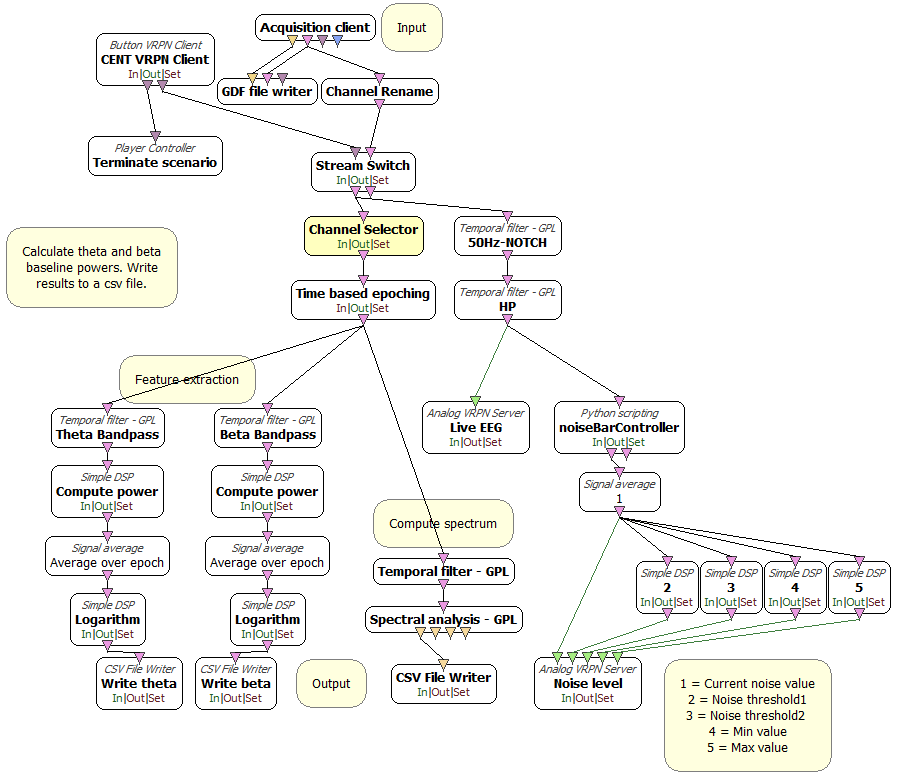
\includegraphics[scale=0.3]{baseline.png}
	\caption{OpenViBE scenario for baseline measurement.}
\end{figure}  

\paragraph{Generate configuration}
Configuration generation scenario is a utility tool used to generate configuration files for the feature extraction in the game trial. The scenario displays no data and the execution only lasts seconds. The scenario takes the baseline values calculated in the previous section and uses them to automatically configure the main game trial. Figure \ref{configuration} displays the corresponding OpenViBE implementation.

\begin{figure}[h]
	\centering
	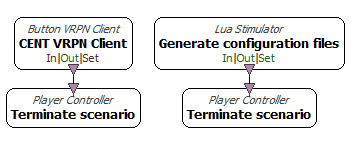
\includegraphics[scale=0.4]{config.png}
	\caption{OpenViBE scenario for writing configuration files.}\label{configuration}
\end{figure}  

\paragraph{Game}
Game scenario evaluates the current mental state of the patient and send information back to CENT. The scenario calculates power values for theta and beta using 1 second epochs and compares them to the values calculated during baseline measurement. The game scenario does not actually do anything related to the game as the actual game mechanics are handled by an external plugin. The OpenViBE implementation of the game trial is visible in figure \ref{gametrial}

\begin{figure}[h]
	\centering
	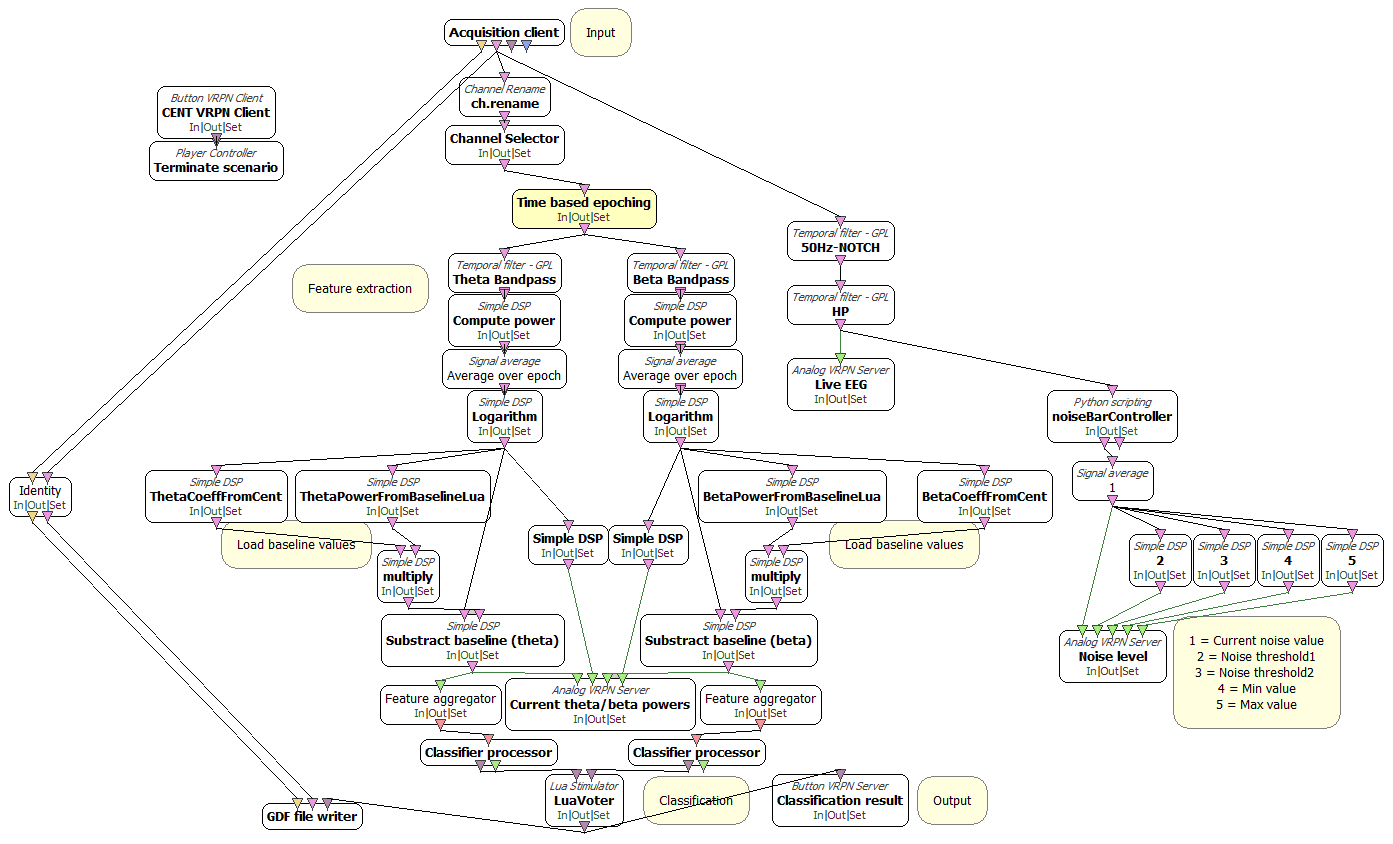
\includegraphics[scale=0.3]{game.png}
	\caption{OpenViBE scenario for the game trial.}\label{gametrial}
\end{figure}
  
\subsection{Signal Processing Protocol}
Neurofeedback signal processing protocol is closely related to the protocol used with brain-computer interfaces (BCI). It thus follows that the signal processing operations performed in a neurofeedback session can be described by borrowing terminology from the field of BCI. In BCI a typical signal processing protocol is divided into four different steps: preprocessing, feature extraction, classification and translation. Preprocessing consists of removing noise and other artifacts from the signal. Feature extraction removes unecessary parts of the signal and classification assigns one of the predefined classes to the incoming signal. Finally the translation performs the action related to the assigned class (such as moving a cursor etc.). In neurofeedback instead of a translation a feedback signal is sent back to the patient i.e, the game reacts to the current neural state. Different signal processing sections of the game scenario have been highlighted in figure \ref{processingsections}. The operation of each section is covered in the following sections.

\begin{figure}[h]
	\centering
	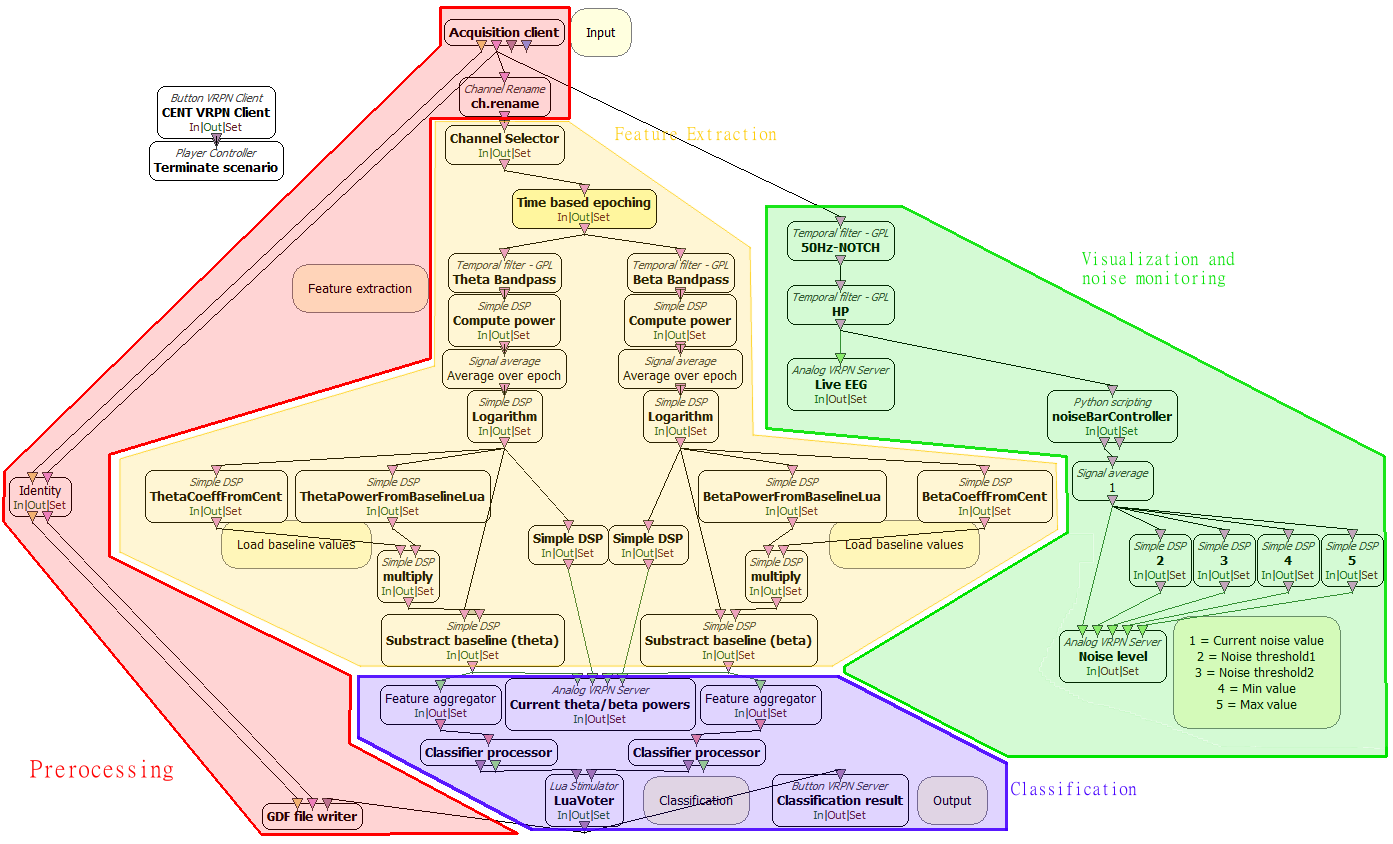
\includegraphics[scale=0.3]{sections.png}
	\caption{Signal processing sections of the game scenario.}\label{processingsections}
\end{figure}

\paragraph{Preprocessing}
The EEG signal is passed into OpenViBE through a custom acquistion driver provided by the manufacturer of the EEG device. This driver can send both the EEG data and Stimulation messages to OpenViBE. The EEG device (Enobio) samples the data with internal sampling rate of 250 Hz which is then passed as packages containing several samples to the OpenViBE. The packet size in OpenViBE terminlogy is called a 'chunk' and the size of the chunk can be specified in the software. Multiple chunks can be combined in an epoch of specified length in seconds. Almost all of the OpenViBE scenarios start from the 'Acquisition client'-box which receives data from the acquistion server running under CENT. Acquisition is not a separate scenario but a part of all the signal processing scenarios of the CENT system. Incoming EEG signal is also saved to a GDF file for later analysis. In addition to the data, also the resulting classification labels (stimulations) are registered for each epoch. None of the filters used in visualization or feature extraction are applied to the saved data.

\paragraph{Visualization and noise measurement}
Visualization and noise measurement is used in all of the signal processing scenarios (with the exception of configuration writing). The EEG signal is transmitted from OpenViBE to CENT using a analog VRPN server. Because the EEG signal picks up a lot of noise originating from physiology and the surroundings two filters are applied. First one removes the 50Hz power line interference using a butterworth notch filter (order: 4, stop band: 40-60Hz). Second filter removes the low frequencies physiological artifacts and signal drift. Second filter is a 4th order high pass with a cut-off frequency of 0.5Hz. Noise monitoring is implemented as a separate Python box which provides information to the current signal quality.

\paragraph{Feature extraction}
Feature extraction, in BCI terminology, means extracting the parts of the incoming signal that contain the information relevant to the task. Feature extraction can be thought of as dimensionality reduction where unnecessary components of the signal are removed in order to improve the classifcation accuracy and robustness. In CENT system both the baseline and game scenario have feature extraction structures. In the baseline scenario feature extraction calculates the power of theta and beta bands. Game scenario also computes the two power values but in addition it also compares these values to the baseline values.

Features are extractred from 500ms segments of EEG with 500ms interval. Power values for the two bands in each epoch are extracted using two 4th-order IIR butterworth filters. By default the passbands are the literary values for theta and beta. Alternatively, the two bands can be configured according to the individual alpha frequency of the patient by using configuration files. The use of individual alpha peak frequency is discussed in section NN. Once the incoming signals have been filtered the voltage values are squared and averaged over the epoch. Finally a logarithm is taken to produce the final power values.  

\paragraph{Classification}
Classification assigns the extracted features to one predefined class according to a predefined mathematical rule. In CENT system these classes are ADHD and not-ADHD and the classification is done with 1D Linear Discriminant Analysis (LDA) classifier. Both of the extracted features are classified as either OVTK\_StimulationId\_Target (for not-ADHD) and OVTK\_StimulationId\_NonTarget (for ADHD). Because the version of OpenViBE used in CENT only supports binary classifiers (classifiers with only two possible outputs) the two classifier outputs are combined using a voting classifier implemented in Lua script (luaVoter.lua). 

\subsection{System Configuration}
As stated earlier the parameters of the signal processing protocol can be configured using XML formatted configuration files. Configuration files can be found in the IEP directory. The adjustable parameters are listed below along with a description of what they do.

\paragraph{Box configuration}

\begin{description}
\item[noiseBarController] Can set parameters for noise detection. Adjustable parameters are EOG threshold and EOG window. Noise detection is also capable of detecting EMG activity but this feature is not currently used.
\item[Time Based Epoching] Can set the duration of EEG  epochs used in classification. Default value is 500ms with 500ms interval between epochs. Epoch length defines the amount of data used for each classification but also sets the interval of feedback to the patient
\item[Theta/Beta Bandpass] Can adjust the bandpass filters used to calculate powers in theta and beta bands. See IAF section for configuring the passbands according to the individual alpha frequency.
\item[Classifier processor] Can change the classification algorithm and parameters for the two classification processors. The two currently supported algorithms are Linear discriminant analysis and Support vector machines. 
\end{description}

\subsection{Individual alpha frequency}
In EEG literature the oscillatory activity of the brain is divided into different frequency ranges denoted by letters from the greek alphabet. The activity in different frequency bands correlates to different mental activities. These values, however, represent a grand average over a large population and might not produce the best possible result in neurofeedback when applied to an individual subject. Earlier research suggests that individual variations in the frequency ranges exist among subjects and there is a method for assigning individual frequency bands for different subjects \cite{klimesch1999eeg}. 

\begin{figure}[ht]
	\centering
	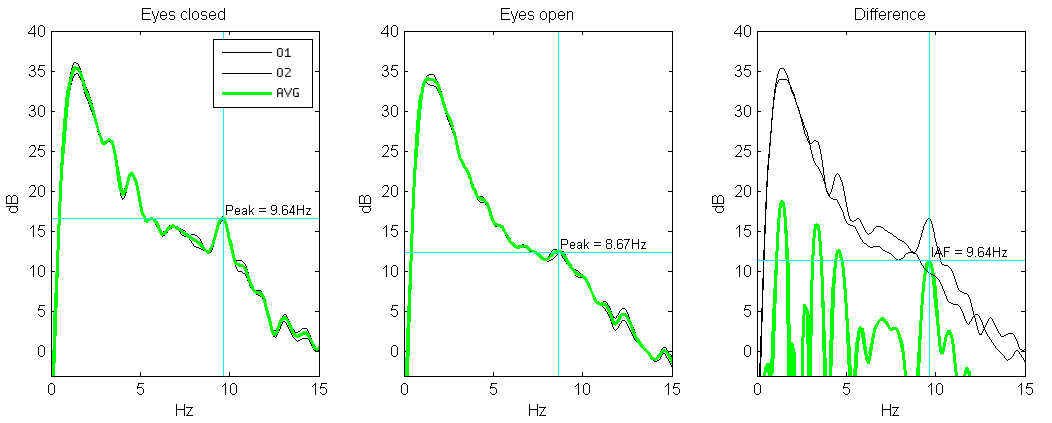
\includegraphics[scale=0.6]{IAF.png}
	\caption{One method for calculating the individual alpha frequency (IAF).}
\end{figure}

In CENT signal analysis individual frequency bands will be determined in the preliminary calibration session of the CENT system to a particular subject. Calibration will consists of recording EEG in eyes-closed condition for few minutes and then analysing the data with an IAF tool also provided in the software package. Alpha peak is extracted from the data by first computing the spectrum and then looking for a peak value in the 7-14 Hz range. Once the peak value has been found other frequency bands can be computed, relative to this peak value (for more details regarding this method see \cite{babiloni2010reactivity}). Once IAF corrected frequency bands have been calculated they can be written into a OpenViBE box configuration files and used in feature extraction. Should the IAF frequency bands not be available or if the calibration fails, frequency bands from the literature are used instead.
